\section{Gravitational Field}
\subsection{Gravitational force}
\begin{defn}{Newton's Law of Gravitation}{}
Gravitational force of attraction between two \underline{point masses} is directly proportional to the product of their masses and inversely proportional to the square of \underline{separation} between their centres.
\begin{equation} \va{F}_g = -\frac{GMm}{r^2}\hat{r} \end{equation}
where gravitational constant $G = 6.67 \times 10^{-11}$ \unit{kg^{-1}.m^3.s^{-2}}
\end{defn} 

\begin{itemize}
    \item The sign is negative due to the attractive nature of gravitational force. (The negative sign is ignored when only the magnitude of the force is required.)
    \item The gravitational forces between two masses are an action-reaction pair; they are equal in magnitude, opposite in direction, and act along the line joining the two point masses.
    \item \textbf{Point masses} have their masses concentrated at one point. Two objects can be considered point masses when they are placed \emph{sufficiently far apart} such that their \emph{dimensions} become negligible compared to the \emph{distance} separating them.
\end{itemize}

\subsection{Gravitational field}
\begin{defn}{Gravitational field}{}
\underline{Region of space} where a mass experiences gravitational force.
\end{defn}

\begin{itemize}
    \item A field of force is a region of space where they may be a \emph{non-contact} force acting on an object placed in that field due to interaction between the field's property and the object's property.
    \item Field lines are used to indicate the direction of a field of force. Density of field lines corresponds to strength of field. (Field lines never touch or cross.)
    \item Gravitational field around Earth is non-uniform (field strength is stronger near Earth, weaker further away from Earth). Field lines are drawn radially pointing towards the centre of Earth.
    \item Gravitational field near Earth's surface is uniform (field strength is the same at all points). Field lines are drawn parallel to each other and of equal spacing.
\end{itemize}

\begin{defn}{Gravitational field strength $g$}{}
Gravitational force per unit mass exerted on a \emph{small test mass} placed at that point.
\begin{equation}
\va{g} = \frac{\va{F}}{m} = -\frac{GM}{r^2}\hat{r} 
\end{equation}
This means that the gravitational field is a inverse square field.
\end{defn} 

\deriv{See Appendix for the derivation.}

This expression refers to the gravitational field created by mass $M$ in its surrounding region of space, where a gravitational force acts on mass $m$.

\begin{itemize}
\item The sign is negative due to the attractive nature of gravitational force acting on a mass in the field. (The negative sign is ignored when only the magnitude is required.)
\item A \textbf{neutral point} refers to the point at which the resultant gravitational field due to surrounding masses is zero.
\begin{figure}[H]
    \centering
    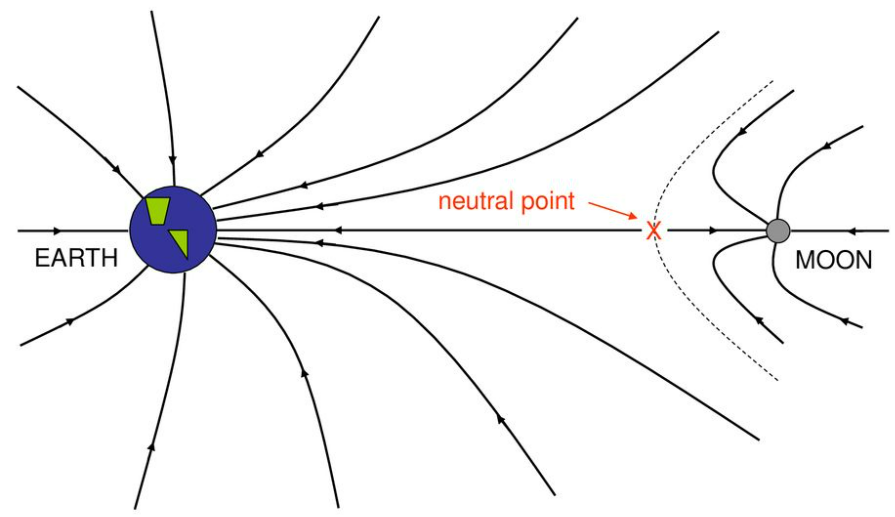
\includegraphics[width=12cm]{images/Neutral_point.png}
    \end{figure}
\end{itemize}

Near the surface of Earth, $g$ can be approximated to have a constant value of $\mathbf{9.81}$ \unit{N.kg^{-1}}, equal to the acceleration of free fall.
\pagebreak

\subsection{Gravitational potential energy}
\begin{defn}{Gravitational potential energy $U$}{}
\underline{Work done} by an \underline{external force} in bringing a \underline{small test mass} from infinity to that point.
\begin{equation} U = -\frac{GMm}{r} \end{equation}
\end{defn}

\begin{itemize}
\item Note that the negative sign cannot be omitted.
\item Maximum $U$ is defined to be 0 at $r=\infty$, hence $U$ is negative.
\item Work done is negative as force and displacement act in opposite directions, hence $U$ is negative.
\end{itemize}

\begin{defn}{Gravitational potential $\phi$}{}
Work done per unit mass by an external force in bringing a small test mass from infinity to that point.
\begin{equation} \phi = \frac{U}{m} = -\frac{GM}{r} \end{equation}
\end{defn}

\begin{itemize}
\item Note that the negative sign cannot be omitted.
\item For the same reasons as above, $\phi$ is negative.
\end{itemize}
\pagebreak

\subsection{Relationship summary}
\begin{figure}[H]
    \centering
    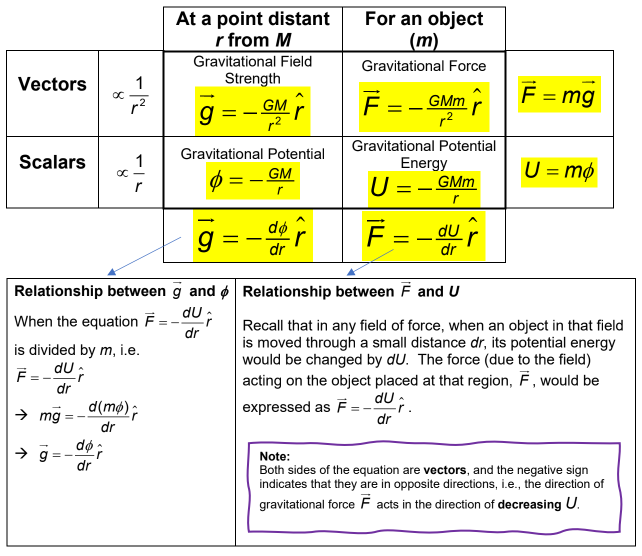
\includegraphics[width=\textwidth]{images/g_field_relationship_summary.png}
\end{figure}
\pagebreak

\subsection{Graphs}
\subsubsection{Force-distance}
Force-distance graph (point mass):
\begin{figure}[H]
\centering
      \begin{tikzpicture}[scale=.4] 
        \draw[->] (-10, 0) -- (10, 0) node[right] {$r$};
        \draw[->] (0, -10) -- (0, 5) node[above] {$\va{F}_g$};
        \draw[color=red, domain=-10:-1,samples=200] plot[id=x1] function{10/x};
        \draw[color=red, domain=1:10,samples=200] plot[id=x2] function{-10/x};
    \end{tikzpicture}
\end{figure}

Force-distance graph (planet):
\begin{figure}[H]
\centering
      \begin{tikzpicture}[scale=.4] 
        \draw[->] (-10, 0) -- (10, 0) node[right] {$r$};
        \draw[->] (0, -10) -- (0, 5) node[above] {$\va{F}_g$};
        \draw[color=red, domain=-10:-2,samples=200] plot[id=x1] function{10/x};
        \draw[color=red, domain=2:10,samples=200] plot[id=x2] function{-10/x};
        \draw[color=red,domain=0:2,samples=200] plot[id=x3] function{-2.5*x};
        \draw[color=red,domain=-2:0,samples=200] plot[id=x3] function{2.5*x};
        \draw[color=black] (0,0) circle (2.0);
    \end{tikzpicture}
\end{figure}
\pagebreak

\subsubsection{Field-distance}
Field-distance graph (point mass)
\begin{figure}[H]
\centering
    \begin{tikzpicture}
    \begin{axis}%
    [axis lines=middle,
     enlargelimits={abs=0.2},
     xlabel = $r$,
     ylabel = $\va{g}$,
     ticks=none
    ]
   \addplot[domain=1:10,samples=200,smooth,red] {-1/x};
   \addplot[domain=-10:-1,samples=200,smooth,red] {-1/x};
    \end{axis}
    \end{tikzpicture}
\end{figure}

Field-distance graph (planet)
\begin{figure}[H]
\centering
    \begin{tikzpicture}
    \begin{axis}%
    [axis lines=middle,
     enlargelimits={abs=0.2},
     xlabel = $r$,
     ylabel = $\va{g}$,
     ticks=none
    ]
   \addplot[domain=1:10,samples=200,smooth,red] {-10/x};
   \addplot[domain=-10:-1,samples=200,smooth,red] {-10/x};
   \draw (axis cs:0,0) circle [radius=1];
   \addplot[mark=none, black,thick, dotted] coordinates {(-1,10) (-1,0)};
   \addplot[mark=none, black,thick, dotted] coordinates {(1,-10) (1,0)};
   \addplot[mark=none, red,thick] coordinates {(-1,10) (1,-10)};
    \end{axis}
    \end{tikzpicture}
\end{figure}

Field-distance graph between two masses
\begin{figure}[H]
\centering
\begin{tikzpicture}
  \begin{axis}%
    [axis lines=middle,
     enlargelimits={abs=0.2},
     xlabel = $r$,
     ylabel = $\va{g}$,
     ticks=none
    ]
   \addplot[domain=0:5,samples=50,smooth,red] {-1/x + 0.2};
%   \addplot[domain=5:9.5] {-1/(x-10) - 0.2}
  \end{axis}
\end{tikzpicture}
\end{figure}
\pagebreak

\subsubsection{Energy-distance}
Energy-distance graph (point mass)
\begin{figure}[H]
\centering
    \begin{tikzpicture}
    \begin{axis}%
    [axis lines=middle,
     enlargelimits={abs=0.2},
     xlabel = $r$,
     ylabel = $U$,
     ymax = 0,
     ticks=none
    ]
   \addplot[domain=1:10,samples=200,smooth,red] {-1/x};
   \addplot[domain=-10:-1,samples=200,smooth,red] {1/x};
    \end{axis}
    \end{tikzpicture}
\end{figure}

Energy-distance graph (planet)
\begin{figure}[H]
\centering
    \begin{tikzpicture}
    \begin{axis}%
    [axis lines=middle,
     enlargelimits={abs=0.2},
     xlabel = $r$,
     ylabel = $U$,
     ymax = 2,
     ticks=none
    ]
   \addplot[domain=1:7,samples=200,smooth,red] {-10/x};
   \addplot[domain=-7:-1,samples=200,smooth,red] {10/x};
   \draw (axis cs:0,0) circle [radius=1];
   \addplot[mark=none, black,thick, dotted] coordinates {(1,-10) (1,0)};
   \addplot[mark=none, black,thick, dotted] coordinates {(-1,-10) (-1,0)};
    \end{axis}
    \end{tikzpicture}
\end{figure}

Energy-distance of satellite (GPE, KE, TE)
\begin{figure}[H]
\centering
\begin{tikzpicture}
    \begin{axis}%
    [axis lines=middle,
     enlargelimits={abs=0.2},
     xlabel = $r$,
     ylabel = $U$,
     xmin = -2,
     ticks=none
    ]
   \addplot[domain=1:10,samples=200,smooth,red] {-10/x};
   \addplot[domain=1:10,samples=200,smooth,blue] {5/x};
   \addplot[domain=1:10,samples=200,smooth,darkgray] {-5/x};
    \end{axis}
\end{tikzpicture}
\end{figure}
\pagebreak

\subsubsection{Potential-distance}
Potential-distance graph (point mass)
\begin{figure}[H]
\centering
    \begin{tikzpicture}
    \begin{axis}%
    [axis lines=middle,
     enlargelimits={abs=0.2},
     xlabel = $r$,
     ylabel = $\phi$,
     ymax = 2,
     xmin = -2,
     ticks=none
    ]
   \addplot[domain=1:12,samples=200,smooth,red] {-10/x};
    \end{axis}
    \end{tikzpicture}
\end{figure}

Potential-distance graph (planet)
\begin{figure}[H]
\centering
    \begin{tikzpicture}
    \begin{axis}%
    [axis lines=middle,
     enlargelimits={abs=0.2},
     xlabel = $r$,
     ylabel = $\phi$,
     ymax = 2,
     xmin = -2,
     ticks=none
    ]
   \addplot[domain=1:12,samples=200,smooth,red] {-10/x};
   \draw (axis cs:0,0) circle [radius=1];
   \addplot[mark=none, black,thick, dotted] coordinates {(1,-10) (1,0)};
    \end{axis}
    \end{tikzpicture}
\end{figure}

Potential-distance graph between two masses
\begin{figure}[H]
\centering
\begin{tikzpicture}
    \begin{axis}%
    [axis lines=middle,
     enlargelimits={abs=0.2},
     xlabel = $r$,
     ylabel = $\phi$,
     ticks=none
    ]
    
    \end{axis}
\end{tikzpicture}
\end{figure}
\pagebreak

\subsection{Applications}
\subsubsection{Orbit velocity}
For a satellite of mass $m$ orbiting a planet of mass $M$ at a certain orbital velocity, \textbf{gravitational force provides centripetal force}.
\begin{align*}
F_g &= F_c \\
\frac{GMm}{r^2} &= \frac{mv^2}{r}
\end{align*}
\[ \boxed{v = \sqrt{\frac{GM}{r}}} \]

\subsubsection{Kinetic energy}
For a satellite in orbit, \textbf{gravitational force provides centripetal force}.
\[ \frac{GMm}{r^2}=\frac{mv^2}{r} \implies mv^2=\frac{GMm}{r} \implies \frac{1}{2}mv^2=\frac{GMm}{2r} \]
\[ \boxed{\mathrm{KE}=\frac{GMm}{2r}} \]

\subsubsection{Kepler's Third Law}
\vocab{Kepler's Third Law} states that the ratio of the square of a body's orbital period to the cube of the axis of orbit is the same for all objects orbiting the same primary.
\begin{equation} T^2 \propto r^3 \end{equation}

\begin{proof}[Derivation]
\textbf{Gravitational force provides centripetal force.}
\[ \frac{GMm}{r^2} = mr \omega ^2 = mr\left(\frac{2 \pi}{T}\right)^2 \]
Making period $T$ the subject, 
\[ T^2 = \frac{4 \pi ^2}{GM} r^3 \implies \boxed{T^2 \propto r^3} \]
\end{proof}

\subsubsection{Escape speed}
\textbf{Escape speed} refers to the \underline{minimum} speed required to escape the effect of a gravitational field.

By conservation of energy,
\[ \text{KE}_i + U_i = \text{KE}_f + U_f \]
At infinity, $U_f = 0$ (by definition of gravitational potential energy) and $\text{KE}=0$ (by definition of escape speed).
\[ \frac{1}{2} mv^2 + \brac{-\frac{GMm}{r}} = 0 \]
Making $v$ the subject,
\[ \boxed{v = \sqrt{\frac{2GM}{r}}} \]

\subsubsection{Geostationary satellite}
\begin{defn}{Geostationary satellite}{}
A satellite that \underline{appears stationary} when observed from a \underline{fixed location} from Earth.
\end{defn}

Characteristics:
\begin{enumerate}
\item Orbital period is the same as the rotational period of Earth about its axis, i.e. $T = 24$ \unit{hr}.
\item Moves in the same direction as the rotation of Earth about its own axis, i.e. from west to east.
\item Vertically above the equator, so that its axis of rotation is the same as the Earth.
    \begin{itemize}
    \item Gravitational force by Earth is the resultant force that provides centripetal force for the satellite. 
    \item Gravitational force is directed towards centre of \underline{Earth}, centripetal force is directed towards centre of \underline{orbit},
    \item so centre of orbit must be centre of Earth.
    \end{itemize}
\end{enumerate}
\pagebreak
\subsubsection{Binary star system}
In a binary star system, two stars rotate about their \emph{common} centre of mass.
\begin{figure}[H]
	\centering
	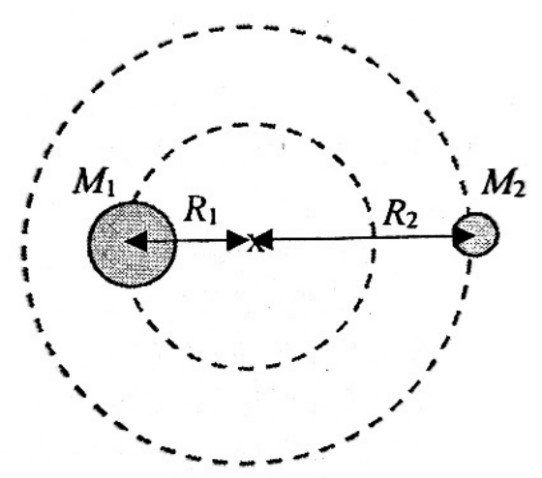
\includegraphics[width=6cm]{Binary_stars}
\end{figure}
For mass $M_1$, gravitational force provides centripetal force for orbit.
\begin{align*}
F_g &= F_c \\
\frac{GM_1M_2}{(R_1+R_2)^2} &= M_1R_1\omega^2 \\
\frac{GM_2}{(R_1+R_2)^2} &= R_1\omega^2
\end{align*}
For mass $M_2$, gravitational force provides centripetal force for orbit.
\begin{align*}
F_g &= F_c \\
\frac{GM_1M_2}{(R_1+R_2)^2} &= M_2R_2\omega^2 \\
\frac{GM_1}{(R_1+R_2)^2} &= R_2\omega^2
\end{align*}
Adding the two equations gives us the period of rotation:
\[ \frac{G(M_1+M_2)}{(R_1+R_2)^2} = (R_1+R_2)\brac{\frac{2\pi}{T}}^2 \]
\[ \boxed{T = \sqrt{\frac{4\pi^2(R_1+R_2)^3}{G(M_1+M_2)}}} \]
\pagebreak

\subsection{Problems}
\begin{prbm}
Explain, in words, why there is a neutral point between two planets.
\end{prbm}
\begin{proof}[Answer]

\end{proof}

\begin{prbm}
At a point on the surface of a uniform sphere of diameter $d$, the gravitational field due to the sphere is $X$. What would be the corresponding value on the surface of a uniform sphere of the same density but of diameter $2d$?
\end{prbm}

\begin{proof}[Solution]
\[ g=\frac{GM}{r^2}=\frac{G\rho\brac{\frac{4}{3}\pi r^3}}{r^2}=\frac{4}{3}G\rho\pi r=\frac{2}{3}G\rho\pi d \implies g \propto d \]
\[ \frac{g_2}{g_1}=\frac{d_2}{d_1} \implies g_2=\frac{2d}{d}X=2X \]
\end{proof}

\begin{prbm}
Assume that the Earth is a point mass of $6.0\times10^{24}$ \unit{kg} and the Moon is a point mass of $7.4\times10^{22}$ \unit{kg}. The distance between them is $3.8\times10^5$ \unit{km}. 

Determine the position of a point from Earth where the gravitational field strength due to Earth and Moon is zero.
\end{prbm}

\begin{proof}[Solution]
Let $x$ be the distance from Earth to the point where the resultant gravitational field strength is zero.

At that point, gravitational field strength due to Earth $g_E$ (directed towards Earth) is \emph{balanced} by gravitational field strength due to Moon $g_M$ (directed towards Moon).
\begin{align*}
g_E &= g_M \\
\frac{GM_E}{x^2} &= \frac{GM_M}{\brac{3.8\times10^8-x}^2} \\
\frac{6.0\times10^{24}}{x^2} &= \frac{7.4\times10^{22}}{\brac{3.8\times10^8-x}^2} \\
\brac{\frac{3.8\times10^8-x}{x}}^2 &= \frac{7.4\times10^{22}}{6.0\times10^{24}} \\
\frac{3.8\times10^8}{x}-1 &= \sqrt{\frac{7.4\times10^{22}}{6.0\times10^{24}}}
\end{align*}
Solving this gives us $x=3.4\times10^8$ \unit{m}.
\end{proof}
\begin{remark}
Remember this way to solve similar questions (do not solve quadratically).
\begin{itemize}
\item Move $x$ to one side.
\item Take square root to reduce it to a linear equation.
\end{itemize}
\end{remark}
\pagebreak

\begin{prbm}[2014 P1 Q13]
X and Y are two stars of equal mass. The points P and Q are equidistant from X and Y.

Which graph best shows the variation in magnitude of the total gravitational field strength $g$ due to the stars when moving from P to Q?
\end{prbm}

\begin{proof}[Answer]

\end{proof}

\begin{prbm}[2015 P1 Q12]
A meteorite of mass $m$ initially has zero velocity relative to a planet. The meteorite falls from a large distance to the planet of mass $M$ and radius $R$. The planet has no atmosphere.

The graph shows the potential $\phi$ of the meteorite in the gravitational field at a distance $r$ from the centre of the planet.

Which expression is equal to the maximum kinetic energy of the meteorite as it hits the surface?
\end{prbm}

\begin{proof}[Answer]

\end{proof}

\begin{prbm}[2018 P1 Q11]

\end{prbm}

\begin{prbm}[2015 P2 Q4]
The planet Jupiter has many moons. Explain why the gravitational field strength at the position of each moon has the same magnitude and direction as the centripetal acceleration of the moon.
\end{prbm}

\begin{proof}[Answer] \ {\\}
The attractive gravitational force exerted by Jupiter on each moon \underline{provides} the centripetal force required to sustain the circular motion about the centre of Jupiter.

The gravitational field strength at each moon's respective position, which is its gravitational force per unit mass, acts towards the centre of Jupiter.

Therefore, each moon's centripetal acceleration, which is its centripetal force per unit mass, must have the same magnitude as its gravitational force per unit mass as well as direction also towards the centre of Jupiter.
\end{proof}

\begin{prbm}[2017 P2 Q2]
Charon is one of the moons of Pluto. When viewed from above, Pluto and Charon rotate in the same direction about their axes.

A space probe on the surface of Pluto is able to observe Charon over a time of several days. Suggest what the space probe observes as a result of
\begin{enumerate}[label=(\roman*)]
\item the period of rotation of Pluto about its axis equalling the orbital period of Charon,
\item equal periods of rotation about their axes for both Pluto and Charon.
\end{enumerate}
\end{prbm}

\begin{proof}[Answer] \
\begin{enumerate}[label=(\roman*)]
\item The space probe observes Charon continuously if Charon orbits in the same direction as Pluto, and periodically if they orbit in opposite directions.
\item The space probe observes the same view of Charon's surface continuously as Charon's synchronous orbit about Pluto causes its near side to face the space probe permanently.
\end{enumerate}
\end{proof}
\pagebreak